
\chapter{Week11}

\section{Wednesday}\index{week7_Tuesday_lecture}
\paragraph{Announcement}
Our second quiz will happen next Friday (November 30), from 1:00 to 2:20 pm in the room Zhiren 205. The \emph{emphasis} will be the content after the mid-term.

\subsection{Recap}
Given a function $f:\mathbb{R}^m\to\mathbb{R}$, suppose $\bm x_0\in\mathbb{R}^m$. The point $\bm x_0$ is said to be a critical point if $Df(\bm x_0)=0$, i.e., $\frac{\partial f}{\partial x_j}(\bm x_0)=0$, $j=1,2,\dots,m$.
\begin{definition}[Critical Point]
The point $\bm x_0\in\mathbb{R}^m$ is said to be a critical point of $f:\mathbb{R}^m\to\mathbb{R}^n$ if the Jacobian matrix at $\bm x=\bm x_0$
\[
Df(\bm x_0)=\begin{pmatrix}
\frac{\partial f_1}{\partial x_1}&
\cdots&\frac{\partial f_1}{\partial x_m}\\
\vdots&\ddots&\vdots\\
\frac{\partial f_n}{\partial x_1}&\cdots&
\frac{\partial f_n}{\partial x_m}
\end{pmatrix}_{n\times m}
\]
is \emph{rank deficient}, i.e., $\rank(Df(\bm x_0))<\min\{n,m\}$.
\end{definition}
Perhaps many classmates are confused with the size and notation of multi-variate formulas. Let's raise some rules to help you minimize errors:
\begin{enumerate}
\item
Any vector is viewed as a column vector
\item
The gradient $\nabla f$ of a scalar function of $n$-argument $f:\mathbb{R}^n\to\mathbb{R}$ is also viewed as a column vector.
\item
The Jacobian matrix $Df$ of a vector function $f:\mathbb{R}^n\to\mathbb{R}^m$ with components $f_1,\dots,f_m$ is the $m\times n$ matrix whose rows are the transposed vectors $\nabla\trans f_1,\dots,\nabla\trans f_m$, i.e., 
\[
Df=\begin{pmatrix}
\nabla\trans f_1\\\vdots\\\nabla\trans f_m
\end{pmatrix}
\]
\end{enumerate}

\begin{theorem}[Sufficient Optimality Condition]
Given a function $f:U(\bm x_0)(\subseteq\mathbb{R}^m)\to\mathbb{R}$, suppose $\bm x_0$ is a critical point, then
\begin{enumerate}
\item
If the Hessian matrix $\left(\frac{\partial^2f}{\partial x_i\partial x_j}(\bm x_0)\right)\succ0$, then $\bm x_0$ is the local minimum
\item
If the Hessian matrix $\left(\frac{\partial^2f}{\partial x_i\partial x_j}(\bm x_0)\right)\prec0$, then $\bm x_0$ is the local maximum
\item
Otherwise, the Hessian matrix gives no further information.
\end{enumerate}
\end{theorem}
\begin{proof}
Taylor expansion $f(\bm x_0+\bm h)$ at point $\bm x=\bm x_0$:
\[
f(\bm x_0+\bm h)=f(\bm x_0)+\frac{1}{2!}\sum_{i,j=1}^m\frac{\partial^2f}{\partial x_i\partial x_j}(\bm x_0)h_ih_j+o(\|\bm h\|^2),
\]
Then apply the definiteness of Hessian matrix to bound the second term on RHS.
\end{proof}
\begin{example}
Given the function $f(x,y)=x^4+y^4-2x^2$, we have
\[
\nabla f=\begin{pmatrix}
4x(x-1)(x+1)\\4y^3
\end{pmatrix},
\]
which induces three critical points $(-1,0),(0,0),(1,0)$, i.e., candidates for extreme points.
\begin{itemize}
\item
The Hessian matrix is given by:
\[
\bm H=\begin{pmatrix}
12x^2-4&0\\
0&12y^2
\end{pmatrix}
\]

The Hessian matrix evaluated at these critial points might give the further information on extreme points:
\[
\begin{array}{lll}
(-1,0)
&
\begin{pmatrix}
8&0\\0&0
\end{pmatrix}
&
\mbox{positive semi-definite}
\end{array}
\]
Therefore, we cannot determine whether $(-1,0)$ is extreme point or not. Similarly, the Hessian matrix evaluated on the remaining two points are neither PD or ND, thus all these three points cannot be determined to be extreme point or not.
\item
However, by term arrangement,
\[
f(x,y)=x^4+y^4-2x^2=(x^2-1)^2+(y^4-1)\ge0
\]
Thus at $(\pm1,0)$, this function achieves its minimum value, i.e., $(\pm1,0)$ are (strictly) local minimum. At small neighborhood of $(0,0)$, as $h\to0$, $f(h,0)$ is increasing; and $f(0,h)$ is decreasing.
\end{itemize}
\end{example}

\subsection{Introduction to Implicit Function Theorem}
The remaining lecture will discuss the proof of Implicit Function Theorem (IFT), which is an intuitive and elementary style.

\paragraph{Motivation}
The purpose of this theorem is to understand the relation of some variables with others. Let's begin with a simple example. 
\begin{example}
Suppose we have the relation
\begin{equation}\label{Eq:11:1}
F(x,y):=x^2+y^2-1=0
\end{equation}
This relation is just the unit circle, plotted in the Fig~(\ref{fig:11:1}).

This relation shows that the location of $y$ is dependent with $x$. We want to study under which condition can we have the one-to-one relation between $x$ and $y$, say $y=f(x)$. For axample, the relation (\ref{Eq:11:1}) pre-assumes the relation
\[
y=\sqrt{1-x^2}
\]
near the small neighborhood of $x_0$. However, when $x_0=\pm1$, we can not obtain such a one-to-one relation.
\begin{figure}[H]\label{fig:11:1}
\centering
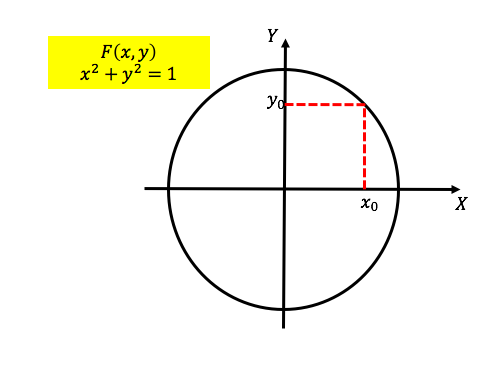
\includegraphics[width=10cm]{week11/F_11_1}
\caption{The set of all points in $\mathbb{R}^2$ satisfying relation (\ref{Eq:11:1})}
\end{figure}
\end{example}
In other words, our interest is to answer the question
\begin{quotation}
How is it possible to find out implicitly, the relation(\ref{Eq:11:1}) can be represented as a one-to-one mapping $y=f(x)$?
\end{quotation}
The IFT gives sufficient condition for that. Moreover, after obtaining a form of function (one-to-one mapping), we could perform something fancy such as differentiation, integration, and otherwise. The IFT also gives the differential form of the function we have obtained.

First let's talk about IFT in two-variable case.
\begin{theorem}[Elementary Version of IFT]\label{The:11:2}
Let $F: U(x_0,y_0)(\subseteq\mathbb{R}^2)\to\mathbb{R}$ be a $\mathcal{C}^p$ ($p\ge1$) function, with
\begin{enumerate}
\item
$F(x_0,y_0)=0$
\item
$\frac{\partial F}{\partial y}(x_0,y_0)\ne0$.
\end{enumerate}
Then there exists a neighborhood of $(x_0,y_0)$, say $I_x\times I_y\subseteq U(x_0,y_0)$ with
\[
\begin{array}{ll}
I_x=\{x\in\mathbb{R}\mid |x-x_0|<\alpha\},
&
I_y=\{y\in\mathbb{R}\mid |y-y_0|<\beta\},
\end{array}
\]
and an \emph{unique} function $f\in\mathcal{C}^p(I_x;I_y)$ satisfying
\begin{align}
F(x,y)&=0\Longleftrightarrow
y=f(x),\qquad
\forall (x,y)\in I_x\times I_y\label{Eq:11:2}\\
f'(x)&=-\frac{\frac{\partial F}{\partial x}}{\frac{\partial F}{\partial y}}(x,f(x))\qquad (=-\frac{F_x}{F_y}(x,f(x)))\label{Eq:11:3}
\end{align}
\end{theorem}
The proof are given below, and we use some diagrams to help you understand it.
\paragraph{Step 1: Applying the continuity of $F$}
w.l.o.g., assume $F_y(x_0,y_0)>0$. Due to the continuity, pick neighbborhood of $(x_0,y_0)$, say $\tilde U(x_0,y_0)$ such that
\begin{equation}
F_y(x,y)>0,\quad
\forall (x,y)\in\tilde U(x_0,y_0)
\end{equation}
\begin{figure}
\centering
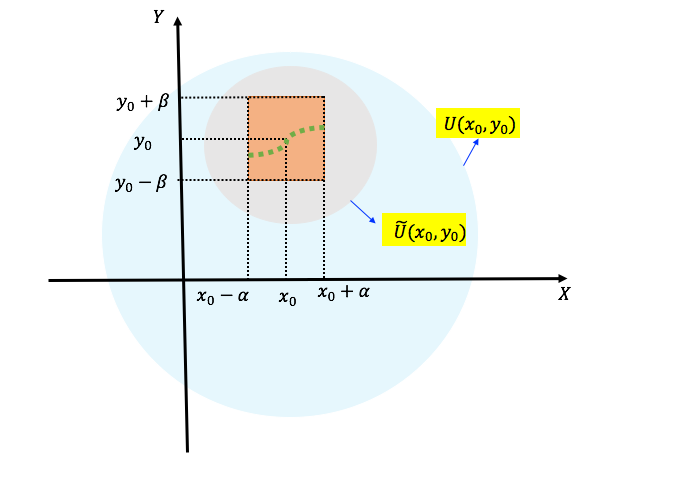
\includegraphics[width=10cm]{week11/F_11_2}
\caption{Interpretation of the constructive proof}
\end{figure}

Pick small $\beta>0$, such that the line segment
\begin{equation}
l:=\{(x_0,y)\mid |y-y_0|<\beta\}\subseteq\tilde U,
\end{equation}
i.e., $F_y>0$ on $l$, which implies $F(x_0,y-\beta)<0$ and $F(x_0,y+\beta)>0$.

By continuity of $F$, there $\exists$ small $\alpha>0$ such that
\begin{align}
\mbox{$F<0$ on $\{(x,y_0-\beta)\mid |x-x_0|<\alpha\}$}\\
\mbox{$F>0$ on $\{(x,y_0+\beta)\mid |x-x_0|<\alpha\}$}
\end{align}

By applying intermediate value theorem, there $\exists$ $y=f(x)$ such that $F(x,y)=0$. Note the the uniqueness of $f$ is guarnteed since $F_y>0$ on $\tilde U(x_0,y_0)$, i.e., the zero of $F$ (on $\tilde U(x_0,y_0)$) is unique for fixed $x$.
\paragraph{Step 2: Show the continuity of $f$ on $I_x$}
Firstly, to show that $f$ is continuous at $x_0$, it suffices to show that for fixed $\varepsilon>0$, 
\begin{equation}\label{Eq:11:8}
\mbox{$\exists\delta>0$ such that $|f(x) - f(x_0)|<\varepsilon$ for $\forall$ $x$ such that $|x-x_0|<\delta$}
\end{equation}
Replace $\beta$ with $\varepsilon$, and pick $\delta:=\alpha$ in step1, the relation (\ref{Eq:11:8}) holds clearly.

To show the continuity of $f$ on the whole interval $I_x$, it suffices to repeat the arguments in step1 by replacing $x_0$ with any other points in $I_x$.

\paragraph{Step3: Show the differentiability of $f$}
For any $x\in I_x$, pick small $\Delta x$ such that $x+\Delta x\in I_x$. Define $y:=f(x)$ and $y+\Delta y:=f(x+\Delta x)$, which follows that
\begin{align}
0&=F(x+\Delta x,y+\Delta y) - F(x,y)\label{Eq:11:9}\\
&=\inp{\nabla F(x+\theta\Delta x,y+\theta\Delta y)}{\begin{pmatrix}
\Delta x\\\Delta y
\end{pmatrix}}\label{Eq:11:10}\\
&=F_x(x+\theta\Delta x,y+\theta\Delta y)\Delta x
+
F_y(x+\theta\Delta x,y+\theta\Delta y)\Delta y\label{Eq:11:11}
\end{align}
where (\ref{Eq:11:9}) is because $F(x+\Delta x,y+\Delta y)=F(x+\Delta x,f(x+\Delta x))$ and then applying (\ref{Eq:11:2}); (\ref{Eq:11:10}) is by applying mean-value theorem ($\theta\in[0,1]$); (\ref{Eq:11:11}) is just term arrangement.

Therefore, solving (\ref{Eq:11:11}) for $\Delta y/\Delta x$, we derive:
\begin{equation}
\frac{\Delta y}{\Delta x}=-\frac{F_x(x+\theta\Delta x,y+\theta\Delta y)}{F_y(x+\theta\Delta x,y+\theta\Delta y)}
\to-\frac{F_x}{F_y}(x,f(x)),
\end{equation}
as $\Delta x\to0$. In other words, $f'=-\frac{F_x}{F_y}(x)$. The differentiability of $f$ is shown thereby.
\paragraph{Alternative approach for evaluating the derivative of $f$}
Once we have the differentiability condition, we could also evaluate the derivative directly.
Note that $\phi(x):=F(x,f(x))=0$ for $\forall x\in I_x$. Differentiating $\phi(x)=0$ both sides leads to
\[
0=\phi'(x)=F_x+F_yf'\qquad\mbox{in }I_x
\]
and therefore $f'=-F_x/F_y$ in $I_x$.
\paragraph{Step4: Show that $f\in\mathcal{C}^p$}
If $p=2$, then the RHS of (\ref{Eq:11:3}) is differentiable w.r.t. $x$, and we find
\[
f''=-\frac{[F_{xx} + F_{xy}\cdot f']F_y - F_x[F_{xy} + F_{yy}\cdot f']}{[F_y]^2}
\]
The case for $p>2$ can be shown by induction.



\begin{theorem}[Simple Generalization]
Let $F(x_1,\dots,x_n;y): U(\bm x_0,y_0) (\subseteq\mathbb{R}^{m+1})\to\mathbb{R}$ be $\mathcal{C}^p$ function with $p\ge1$. Suppose
\begin{enumerate}
\item
$F(\bm x_0,y_0)=0$
\item
$\frac{\partial F}{\partial y}(\bm x_0,y_0)\ne0$
\end{enumerate}

Then there exists a neighborhood of $(x_0,y_0)$, say $I_{\bm x}\times I_y\subseteq U(\bm x_0,y_0)$ with


\[
\begin{array}{ll}
I_{\bm x}=\{\bm x\in\mathbb{R}^m\mid \|\bm x-\bm x_0\|<\alpha\},
&
I_{y}=\{y\in\mathbb{R}\mid |y-y_0|<\beta\},
\end{array}
\]
and an \emph{unique} function $f\in\mathcal{C}^p(I_{\bm x},I_y)$ satisfying
\begin{align}
F(x_1,\dots,x_m,y)&=0\Longleftrightarrow
F(x_1,\dots,x_m,f(\bm x))=0,\qquad
\forall (\bm x,y)\in I_{\bm x}\times I_y\\
\frac{\partial f}{\partial x_j}&=-\frac{\frac{\partial F}{\partial x_j}}{\frac{\partial F}{\partial y}} j=1,\dots,m
\end{align}

\end{theorem}
\begin{proof}
The proof for the case $j=1$ is just by fixing all variables in the functions $F(x_1,\dots,x_m,y)$ except $x_1$ and $y$, and then following the same argument in Theorem(\ref{The:11:2})
\end{proof}







